O menino Araújo, filho de biólogos, sempre foi fascinado pelas espécies de cobras que eram criadas no cativeiro da casa.
 Hoje pela manhã ele ganhou um dominó no bingo da escola e, já em casa, formulou o jogo ``A Maior Cobra Legal de Dominós''.

Uma peça de dominó é um par não ordenado de inteiros $(i,j)$ tal que $0 \leq i, j \leq N$.
Um jogo completo de dominó com $N$ valores é composto por todas as peças de dominós possíveis que tem valores entre $0$ e $N$.
Uma cobra de dominó é uma sequência de peças $(i_1, j_1)(i_2, j_2)\dots(i_m, j_m)$ tal que $j_k = i_{k+1}$ para todo $k$ válido.
O objetivo do jogo de nosso jovem protagonista é bem simples: formar a maior cobra de dominós possível usando peças de um jogo completo.
 Por exemplo, se seu jogo de dominó tem peças com valores de $0$ até 3, uma possível maior cobra de se formar teria 9 peças com a seguinte configuração:

\begin{center}
  $( 0,0 )( 0,1 )( 1,1 )( 1,2 )( 2,2 )( 2,0 )( 0,3 )( 3,3 )( 3,1 )$
\end{center}

Observe que a peça 2-3 (ou 3-2, a peça é a mesma) não foi possível de ser usada.
Por outro lado, se o valor de uma lado de suas peças vai até 4, uma possível maior cobra de se formar teria 15 peças com a seguinte configuração:

\begin{center}
 $( 0,0 )( 0,1 )( 1,1 )( 1,2 )( 2,2 )( 2,0 )( 0,3 )( 3,3 )( 3,1 )( 1,4 )( 4,4 )( 4,2 )( 2,3 )( 3,4 )( 4,0 )$
\end{center}

Curioso que é, o menino Araújo solicitou a ajuda dos programadores da Maratona Mineira para criar um programa com a seguinte missão: dado o valor máximo que pode aparecer em uma peça de dominó, informe qual é o tamanho da maior cobra legal de dominós.


\begin{center}
  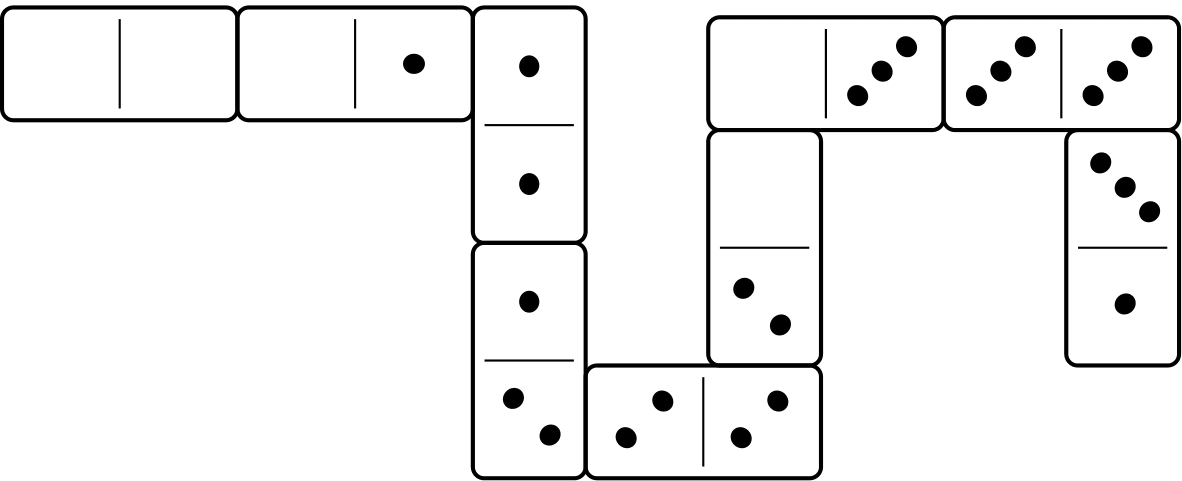
\includegraphics[width=0.7\linewidth]{\CWD/dominos.png}
\end{center}


\section*{Entrada}

A entrada consiste de uma única linha contendo único inteiro $N$, o valor máximo que pode existir em uma peça de dominó.


\section*{Saída}

A saída consiste de um único inteiro, que representa o tamanho da maior cobra de dominó que pode ser formada.


\section*{Restrições}

\begin{itemize}
  \item $0 \leq N \leq 5000$
\end{itemize}

\section*{Exemplos}

\exemplo
